% Options for packages loaded elsewhere
\PassOptionsToPackage{unicode}{hyperref}
\PassOptionsToPackage{hyphens}{url}
%
\documentclass[
  man]{apa7}
\usepackage{amsmath,amssymb}
\usepackage{iftex}
\ifPDFTeX
  \usepackage[T1]{fontenc}
  \usepackage[utf8]{inputenc}
  \usepackage{textcomp} % provide euro and other symbols
\else % if luatex or xetex
  \usepackage{unicode-math} % this also loads fontspec
  \defaultfontfeatures{Scale=MatchLowercase}
  \defaultfontfeatures[\rmfamily]{Ligatures=TeX,Scale=1}
\fi
\usepackage{lmodern}
\ifPDFTeX\else
  % xetex/luatex font selection
\fi
% Use upquote if available, for straight quotes in verbatim environments
\IfFileExists{upquote.sty}{\usepackage{upquote}}{}
\IfFileExists{microtype.sty}{% use microtype if available
  \usepackage[]{microtype}
  \UseMicrotypeSet[protrusion]{basicmath} % disable protrusion for tt fonts
}{}
\makeatletter
\@ifundefined{KOMAClassName}{% if non-KOMA class
  \IfFileExists{parskip.sty}{%
    \usepackage{parskip}
  }{% else
    \setlength{\parindent}{0pt}
    \setlength{\parskip}{6pt plus 2pt minus 1pt}}
}{% if KOMA class
  \KOMAoptions{parskip=half}}
\makeatother
\usepackage{xcolor}
\usepackage{longtable,booktabs,array}
\usepackage{calc} % for calculating minipage widths
% Correct order of tables after \paragraph or \subparagraph
\usepackage{etoolbox}
\makeatletter
\patchcmd\longtable{\par}{\if@noskipsec\mbox{}\fi\par}{}{}
\makeatother
% Allow footnotes in longtable head/foot
\IfFileExists{footnotehyper.sty}{\usepackage{footnotehyper}}{\usepackage{footnote}}
\makesavenoteenv{longtable}
\usepackage{graphicx}
\makeatletter
\def\maxwidth{\ifdim\Gin@nat@width>\linewidth\linewidth\else\Gin@nat@width\fi}
\def\maxheight{\ifdim\Gin@nat@height>\textheight\textheight\else\Gin@nat@height\fi}
\makeatother
% Scale images if necessary, so that they will not overflow the page
% margins by default, and it is still possible to overwrite the defaults
% using explicit options in \includegraphics[width, height, ...]{}
\setkeys{Gin}{width=\maxwidth,height=\maxheight,keepaspectratio}
% Set default figure placement to htbp
\makeatletter
\def\fps@figure{htbp}
\makeatother
\setlength{\emergencystretch}{3em} % prevent overfull lines
\providecommand{\tightlist}{%
  \setlength{\itemsep}{0pt}\setlength{\parskip}{0pt}}
\setcounter{secnumdepth}{-\maxdimen} % remove section numbering
% Make \paragraph and \subparagraph free-standing
\ifx\paragraph\undefined\else
  \let\oldparagraph\paragraph
  \renewcommand{\paragraph}[1]{\oldparagraph{#1}\mbox{}}
\fi
\ifx\subparagraph\undefined\else
  \let\oldsubparagraph\subparagraph
  \renewcommand{\subparagraph}[1]{\oldsubparagraph{#1}\mbox{}}
\fi
\newlength{\cslhangindent}
\setlength{\cslhangindent}{1.5em}
\newlength{\csllabelwidth}
\setlength{\csllabelwidth}{3em}
\newlength{\cslentryspacingunit} % times entry-spacing
\setlength{\cslentryspacingunit}{\parskip}
\newenvironment{CSLReferences}[2] % #1 hanging-ident, #2 entry spacing
 {% don't indent paragraphs
  \setlength{\parindent}{0pt}
  % turn on hanging indent if param 1 is 1
  \ifodd #1
  \let\oldpar\par
  \def\par{\hangindent=\cslhangindent\oldpar}
  \fi
  % set entry spacing
  \setlength{\parskip}{#2\cslentryspacingunit}
 }%
 {}
\usepackage{calc}
\newcommand{\CSLBlock}[1]{#1\hfill\break}
\newcommand{\CSLLeftMargin}[1]{\parbox[t]{\csllabelwidth}{#1}}
\newcommand{\CSLRightInline}[1]{\parbox[t]{\linewidth - \csllabelwidth}{#1}\break}
\newcommand{\CSLIndent}[1]{\hspace{\cslhangindent}#1}
\ifLuaTeX
\usepackage[bidi=basic]{babel}
\else
\usepackage[bidi=default]{babel}
\fi
\babelprovide[main,import]{english}
% get rid of language-specific shorthands (see #6817):
\let\LanguageShortHands\languageshorthands
\def\languageshorthands#1{}
% Manuscript styling
\usepackage{upgreek}
\captionsetup{font=singlespacing,justification=justified}

% Table formatting
\usepackage{longtable}
\usepackage{lscape}
% \usepackage[counterclockwise]{rotating}   % Landscape page setup for large tables
\usepackage{multirow}		% Table styling
\usepackage{tabularx}		% Control Column width
\usepackage[flushleft]{threeparttable}	% Allows for three part tables with a specified notes section
\usepackage{threeparttablex}            % Lets threeparttable work with longtable

% Create new environments so endfloat can handle them
% \newenvironment{ltable}
%   {\begin{landscape}\centering\begin{threeparttable}}
%   {\end{threeparttable}\end{landscape}}
\newenvironment{lltable}{\begin{landscape}\centering\begin{ThreePartTable}}{\end{ThreePartTable}\end{landscape}}

% Enables adjusting longtable caption width to table width
% Solution found at http://golatex.de/longtable-mit-caption-so-breit-wie-die-tabelle-t15767.html
\makeatletter
\newcommand\LastLTentrywidth{1em}
\newlength\longtablewidth
\setlength{\longtablewidth}{1in}
\newcommand{\getlongtablewidth}{\begingroup \ifcsname LT@\roman{LT@tables}\endcsname \global\longtablewidth=0pt \renewcommand{\LT@entry}[2]{\global\advance\longtablewidth by ##2\relax\gdef\LastLTentrywidth{##2}}\@nameuse{LT@\roman{LT@tables}} \fi \endgroup}

% \setlength{\parindent}{0.5in}
% \setlength{\parskip}{0pt plus 0pt minus 0pt}

% Overwrite redefinition of paragraph and subparagraph by the default LaTeX template
% See https://github.com/crsh/papaja/issues/292
\makeatletter
\renewcommand{\paragraph}{\@startsection{paragraph}{4}{\parindent}%
  {0\baselineskip \@plus 0.2ex \@minus 0.2ex}%
  {-1em}%
  {\normalfont\normalsize\bfseries\itshape\typesectitle}}

\renewcommand{\subparagraph}[1]{\@startsection{subparagraph}{5}{1em}%
  {0\baselineskip \@plus 0.2ex \@minus 0.2ex}%
  {-\z@\relax}%
  {\normalfont\normalsize\itshape\hspace{\parindent}{#1}\textit{\addperi}}{\relax}}
\makeatother

\makeatletter
\usepackage{etoolbox}
\patchcmd{\maketitle}
  {\section{\normalfont\normalsize\abstractname}}
  {\section*{\normalfont\normalsize\abstractname}}
  {}{\typeout{Failed to patch abstract.}}
\patchcmd{\maketitle}
  {\section{\protect\normalfont{\@title}}}
  {\section*{\protect\normalfont{\@title}}}
  {}{\typeout{Failed to patch title.}}
\makeatother

\usepackage{xpatch}
\makeatletter
\xapptocmd\appendix
  {\xapptocmd\section
    {\addcontentsline{toc}{section}{\appendixname\ifoneappendix\else~\theappendix\fi\\: #1}}
    {}{\InnerPatchFailed}%
  }
{}{\PatchFailed}
\keywords{employee engagement, scale validation, bifactor structure, organizational surveying\newline\indent Word count: X}
\DeclareDelayedFloatFlavor{ThreePartTable}{table}
\DeclareDelayedFloatFlavor{lltable}{table}
\DeclareDelayedFloatFlavor*{longtable}{table}
\makeatletter
\renewcommand{\efloat@iwrite}[1]{\immediate\expandafter\protected@write\csname efloat@post#1\endcsname{}}
\makeatother
\usepackage{lineno}

\linenumbers
\usepackage{csquotes}
\ifLuaTeX
  \usepackage{selnolig}  % disable illegal ligatures
\fi
\IfFileExists{bookmark.sty}{\usepackage{bookmark}}{\usepackage{hyperref}}
\IfFileExists{xurl.sty}{\usepackage{xurl}}{} % add URL line breaks if available
\urlstyle{same}
\hypersetup{
  pdftitle={Development and validation of an prescriptive bi-factor measure of employee engagement},
  pdfauthor={John Kulas1, Renata Garcia Prieto Palacios Roji2, Casey Osorio-Duffoo3, Mike DeFabiis4, \& Morgan Russell4},
  pdflang={en-EN},
  pdfkeywords={employee engagement, scale validation, bifactor structure, organizational surveying},
  hidelinks,
  pdfcreator={LaTeX via pandoc}}

\title{Development and validation of an prescriptive bi-factor measure of employee engagement}
\author{John Kulas\textsuperscript{1}, Renata Garcia Prieto Palacios Roji\textsuperscript{2}, Casey Osorio-Duffoo\textsuperscript{3}, Mike DeFabiis\textsuperscript{4}, \& Morgan Russell\textsuperscript{4}}
\date{}


\shorttitle{BiFactor Engagement}

\authornote{

Correspondence concerning this article should be addressed to John Kulas, 1 Normal Ave, Montclair, NJ 07043. E-mail: \href{mailto:kulasj@montclair.edu}{\nolinkurl{kulasj@montclair.edu}}

}

\affiliation{\vspace{0.5cm}\textsuperscript{1} eRg\\\textsuperscript{2} PepsiCo\\\textsuperscript{3} Harver\\\textsuperscript{4} Montclair State University}

\abstract{%
The most popular conceptual specification employee engagement implicates sub-dimensions of vigor, dedication, and absorption. The tripartite model of attitudes isolates cognitive, behavioral, and affective components. The current investigation documents the development and validation of an intentionally complex engagement measure - one that intentionally crosses the conceptually substantive and elemental attitude components. An initial item set of 72 were culled to 36 via content validation. These 36 candidate items were piloted with a snowball sample of 330 respondents and reduced to 20. The final 18 items were identified via further administration to 743 Prolific respondents. We finalize the scale definitions for a bifactor engagement measure that is comprised of intentionally complex items. This complexity crosses attitudinal and substantive components. The final scale definition exhibited moderately good bifactor fit, and the final version of the instrument allows aggregations that should be desirable for both researchers (substantive) as well as practitioners (attitude). Construct validation was accomplished via
Criterion-related validation included documented associations with intent to quit, satisfaction, and .
}



\begin{document}
\maketitle

Incorporated:

\begin{itemize}
\tightlist
\item
  \texttt{...Engagement-Survey-Projects/Construct\ Validation}
\end{itemize}

The roots of employee (aka work, e.g., Wilmar B. Schaufeli \& Bakker, 2010a) engagement research likely started with theoretical expansions of forms of employee participation (see, for example, Ferris \& Hellier, 1984) and job involvement (e.g., Elloy, Everett, \& Flynn, 1991). This exploration extended into broader considerations of attitudes and emotions (Staw, Sutton, \& Pelled, 1994) and were informed by further exploration of the dimensionality of constructs such as organizational commitment (Meyer \& Allen, 1991). Staw et al. (1994) investigated the relationships between \emph{positive emotions} and favorable work outcomes, and although they do not use the word, ``engagement'', their distinction between felt and expressed emotion likely held influence upon the burgeoning interest in the engagement construct. The 1990's as a whole can be reasonably characterized as notable regarding the construct's development and refinement William A. Kahn (1990a).

William A. Kahn (1990a) described engaged employees as being physically involved, cognitively vigilant, and emotionally connected. Although occasionally referred to as residing on the opposing pole to \emph{burnout} (Christina Maslach \& Leiter, 2008), these two constructs are currently most commonly conceptualized as being distinct (Goering, Shimazu, Zhou, Wada, \& Sakai, 2017; Kim, Shin, \& Swanger, 2009; Wilmar B. Schaufeli, Taris, \& Van Rhenen, 2008; Timms, Brough, \& Graham, 2012), although certainly not universally (Cole, Walter, Bedeian, \& O'Boyle, 2012; Taris, Ybema, \& Beek, 2017). Goering et al. (2017) conclude that these two constructs have a moderate (negative) association, but also distinct nomological networks. Wilmar B. Schaufeli et al. (2008) investigated both internal and external association indicators, concluding that engagement and burnout (as well as \emph{workaholism}) should be considered three distinct constructs.

Burnout can be defined as a psychological syndrome characterized by exhaustion (low energy), cynicism (low involvement), and inefficacy (low self-efficacy), which is experienced in response to chronic job stressors (e.g., Leiter \& Maslach, 2004; C. Maslach \& Leiter, 1997). Alternatively, engagement refers to an individual worker's involvement and satisfaction as well as enthusiasm for work (James K. Harter, Schmidt, \& Hayes, 2002). William A. Kahn (1990a) defines engagement as ``the harnessing of organization members' selves to their work roles; in engagement, people employ and express themselves physically, cognitively, and emotionally during role performances'' (p.~692).

\hypertarget{engagement-as-an-attitude}{%
\subsection{Engagement as an attitude}\label{engagement-as-an-attitude}}

Clear in its history is the conceptualization of engagement as a work \emph{attitude}. This conceptualization of engagement as an attitude was also heavily influenced by Rosenberg (1960)'s tripartite model of attitudes, which was popular in the 1990's. According to Rosenberg (1960), attitudes are a molar construct with cognitive, affective, and behavioral dimensions. Although falling out of favor in the decades following its construction, interest in the tripartite model was revived by Kaiser and Wilson (2019). It is perhaps currently most prominently embedded within contemporary perspectives on personality (e.g., patterns of thinking, feeling, and behaving). The attitudinal perspectives of engagement eventually blended into perspectives that focused on exploring the engagement construct through the lens of other conceptually similar constructs Shaw (2005).

The first, to our knowledge, use of the word ``engagement'' as a construct came in William A. Kahn (1990b), defining it as: ``the harnessing of organization members' selves to their work roles; in engagement, people employ and express themselves physically, cognitively, and emotionally during role performances.'' Although this definition was quickly bypassed by subsequent papers (see, for example, (Baumruk, 2004) and (Shaw, 2005), who framed it in terms of one's cognitive and affective \emph{commitment} to one's organization), William A. Kahn (1990b)'s definition is notable in that it conforms to the then-ascendant tripartite model of attitudes proposed by Rosenberg (1960). This model frames attitudes as latent variables that manifest cognitively, affectively and behaviorally.

\hypertarget{engagements-substantive-elements}{%
\subsection{Engagement's substantive elements}\label{engagements-substantive-elements}}

W. B. Schaufeli and Bakker (2003)'s elemental description of engagement is perhaps the most contemporarily popular, likely at least partially a function of the popularity of their widely-available (in many different languages) measure, the Utrecht Work Engagement Scale (UWES). schaufeli\_uwesutrecht\_2003 define engagement as a ``positive, fulfilling, work-related state of mind that is characterized by vigor, dedication, and absorption'' (p.~74). Via their specification, vigor is described as high levels of energy and mental resilience while working. Dedication refers to being strongly involved in one's work and experiencing a sense of significance, enthusiasm, inspiration, pride, and challenge. Absorption is characterized by being fully concentrated and happily engrossed in one's work, whereby time passes quickly and one has difficulties with detaching oneself from work (Wilmar B. Schaufeli, Salanova, González-Romá, \& Bakker, 2002). The dimension of absorption has been noted as being influenced in conceptual specification by (Csikszentmihalyi, 1990)'s concept of ``flow''.

\hypertarget{existing-measures-of-engagement}{%
\subsection{Existing Measures of Engagement}\label{existing-measures-of-engagement}}

Regarding measurement, Gallup is widely acknowledged as an early pioneer in the measurement of the construct (see, for example, Coffman \& Harter, 1999). The Utrecht Work Engagement Scale (UWES) is another self-report questionnaire developed by W. B. Schaufeli and Bakker (2003) that directly assesses the vigor, dedication, and absorption elements. Our review of existing instruments non-exhaustively presents measures that are commonly viewed as \emph{either} predominantly academic or applied, although please note that this is an imposed subjective distinction.

\hypertarget{research-measures-e.g.-freely-available.}{%
\subsubsection{Research measures (e.g., freely available).}\label{research-measures-e.g.-freely-available.}}

W. B. Schaufeli and Bakker (2003) characterize engagement as a ``positive, fulfilling, work-related state of mind that is characterized by vigor, dedication, and absorption'' (p.~74). W. B. Schaufeli and Bakker (2003) use this tripartite framework to measure engagement via the Utrecht Work Engagement Scale (UWES).

The Intellectual, Social, Affective (ISA) Engagement Scale (Soane et al., 2012) is another option for researchers. This 9-item measure draws inspiration from William A. Kahn (1990a)'s theory of engagement and can aggregate to three 3-item scales (Intellectual Engagement, Social Engagement, and Affective Engagement) or one 9-item summary aggregate (Overall Engagement). Intellectual engagement refers to the degree of intellectual absorption one has in their work and the degree they think about improving work (Soane et al., 2012). Social engagement primarily concerns social connections in a workplace context as well as having shared values with colleagues (Soane et al., 2012). According to Soane et al. (2012), affective engagement refers to a positive emotional state relating to one's work role. This measure has been explicitly validated at both the subscale and overall aggregate level (Soane et al., 2012).

Another example of an engagement measure comes from Saks (2006), who splits engagement into two distinct entities: job engagement and organization engagement. This dichotomy largely results from William A. Kahn (1990a)'s theory that an individual's role is central to engagement. Saks (2006) further posits that employees typically have more than one role, with the most important being their work role and their role as a member of an organization. The former role is specific to the employee's job, while the latter is more broad and refers to the organization as a whole. Antecedents and consequences of this measure have been tested, with findings suggesting that perceived organizational support precedes both job and organizational engagement and that job satisfaction, organizational commitment, intent to quit, and organizational citizenship behaviors (OCBs) are consequences (Saks, 2006). Recently the broader theoretical model underpinning the measure was revisited and revised to include several new antecedents (e.g.~leadership, job demands, dispositional characteristics, etc.) leading to engagement as well as consequences (e.g.~burnout, stress, health and well-being, etc.) resulting from high or low levels of engagement (Saks, 2019).

\hypertarget{commercial-measures}{%
\subsubsection{Commercial measures}\label{commercial-measures}}

Gallup's Q12 is a popular commercial measure for engagement. The Q12 is a 12-item measure that originated from a push to use ``soft'' metrics as opposed to ``hard'' ones for future action planning (Coffman \& Harter, 1999). In this interpretation ``soft'' metrics tend to be metrics that are more abstract and difficult to measure (e.g.~engagement, brand loyalty), while ``hard'' metrics are easily-measured and typically deal with concrete numbers (e.g.~turnover, profitability). In the original creation of the survey, each of the 12 items were found to relate to important organizational outcomes including productivity, profitability, turnover, and customer satisfaction (Coffman \& Harter, 1999). A recent meta-analysis of 456 studies revealed that the Q12 also relates to additional performance measures such as absenteeism, wellbeing, and organizational citizenship (J. K. Harter, Schmidt, Agrawal, \& Plowman, 2013). While this engagement measure is one of the most popular, some scholars disagree with its conceptualization as ``engagement''; some feel that this measure is better described as (or no different than) a measure of overall satisfaction, as the two concepts are highly correlated, \emph{r} = .91 (Sirota \& Klein, 2013).

Gallup is not the only organization with an engagement measure; many consulting companies have commercially available surveys, models, and processes for measuring engagement. One such example is Aon Hewitt, a consulting firm that annually measures engagement for over 1000 companies worldwide. Their measurements are centered around an engagement model that focuses on three main factors: say, stay, and strive. Essentially, the model states that employees demonstrate engagement through saying positive statements about their organization, staying at their organization for a long time, and striving to put in their best effort and help the organization succeed (Hewitt, 2017). In their most recent analysis. Hewitt (2017) recently noted that global levels of engagement may be declining as in this report they had retracted since the previous year.

BlessingWhite, another consulting firm, provides a different model for engagement. BlessingWhite's model, the X Model, measures engagement through the lens of satisfaction and contribution. Essentially, BlessingWhite believes that cooperation between the organization and individual employees is necessary, and that maximum engagement can only be reached when an employee reaches maximum levels of satisfaction while also outputting maximum contribution towards the organization (BlessingWhite, 2018). Their model holds each level in the organization accountable for employee levels of engagement. From their view, executive leaders must shape the organization's culture, and managers must be able to effectively communicate with and motivate their subordinates (BlessingWhite, 2018).

The last commercial example discussed here\footnote{This non-exhaustive list is not meant to be comprehensive. We intended to present some popular measures (albeit from larger vendors) in an attempt to capture the variety of rationales and purposes behind the creation and administration of these measures.} is the Towers Perrin-ISR, which holds the philosophy that employee engagement can only be worked on indirectly; engagement can only be attained through effective leadership, business strategy, and organizational culture (Ballendowitsch \& Perrin-ISR, 2009). Rather than focus on building an involved model for engagement, Towers Perrin-ISR instead focuses on leadership development and creating a healthy organizational culture. Through fulfilling these antecedents of engagement, Ballendowitsch and Perrin-ISR (2009) argues that employees will have a vivid understanding of organizational goals. In addition, employees will become committed to the organization and motivated to contribute.

\hypertarget{our-measure-of-engagement}{%
\subsection{Our Measure of Engagement}\label{our-measure-of-engagement}}

Our theoretical conceptualization of work engagement is primarily informed by W. B. Schaufeli and Bakker (2003) and Rosenberg (1960). Through the lens of our framework, engagement is a mental state wherein employees: a) feel energized (\emph{Vigor}), b) are enthusiastic about the content of their work and the things they do (\emph{Dedication}), and c) are so immersed in their work activities that time seems compressed (\emph{Absorption})\footnote{This model is not without criticism, however. Some critics question its structural validity by pointing out that vigor, dedication and absorption all correlate highly with each other (Kulikowski, 2017).}.
We further decompose each of these facets into three attitudinal components: d) feeling (e.g., affect), e) thought (e.g., cognition), and f) action (e.g., behavior).

Wilmar B. Schaufeli (2013) stated a preference for the label ``work engagement'' rather than referring to the construct as ``employee engagement'', arguing that the ``employee'' referrent perhaps invites a blurring of definitions with other conceptually similar constructs such as commitment or organizational citizenship. Regarding this distinction between ``the job'' and ``the organization'', our measure scatters indicators of both throughout, although we did not intentionally balance the measure with regard to the referent, as do others, such as Saks (2006).

Our conceptualization of work engagement is a mental state wherein employees: a) feel energized (\emph{Vigor}), b) are enthusiastic about the content of their work and the things they do (\emph{Dedication}), and c) are so immersed in their work activities that time seems compressed (\emph{Absorption}). We further decompose each of these facets into three attitudinal components: d) feeling (e.g., affect), e) thought (e.g., cognition), and f) action (e.g., behavior). Development and construct validation of the focal 18-item measure of engagement is described in Russell, Ossorio Duffoo, Garcia Prieto Palacios Roji, and Kulas (2022) whereas the current study on administrative response cues in the form of order of item presentation. The expectation is that either model (attitudinal or substantive) will exhibit stronger factorial validity when item administration parallels latent structure.

\hypertarget{bifactor-structures.}{%
\subsubsection{Bifactor structures.}\label{bifactor-structures.}}

Methodologically, we have chosen to empirically model our measure via confirmatory factor analysis of a bifactor structure (aka bifactor analysis). Typically, bifactor analyses are utilized when exploring common method variance (Biderman, Nguyen, Cunningham, \& Ghorbani, 2011; Gäde, Schermelleh-Engel, \& Klein, 2017; Reise, 2012), and the ``bi'' construct is a unidimensional specification (e.g., ``one'' construct/factor commonly interpreted as common method oriented). The current study extends this tradition, as two multi-dimensional factor structures specified \emph{a priori} are simultaneously imposed.

\hypertarget{study-1-content-validation}{%
\section{Study 1: Content Validation}\label{study-1-content-validation}}

\hypertarget{study-2-empirical-scale-reduction}{%
\section{Study 2: Empirical Scale Reduction}\label{study-2-empirical-scale-reduction}}

\hypertarget{study-3-construct-and-criterion-validation}{%
\section{Study 3: Construct and Criterion-validation}\label{study-3-construct-and-criterion-validation}}

\hypertarget{methods}{%
\section{Methods}\label{methods}}

We solicited three different samples for purposes of winnowing from 20 to 18 final scale items. One sample was a Prolific panel, one was a Qualtrics panel, and one was a ``snowball'' sample whereby friends and colleagues of the paper authors were invited to participate. In the snowball sample, invited individuals were also asked to further forward the survey along to friends and colleagues of theirs, with the ``forwarding along'' component being requested \emph{ad infinitum}.

\hypertarget{methods-1}{%
\section{Methods}\label{methods-1}}

The present article explores two methods for constructing a scale that incorporates both the substantive and attitudinal models into one, a more classical one based on corrected item-total correlations and one based on modification indices.

\hypertarget{construct-validation}{%
\section{Construct validation}\label{construct-validation}}

The current study's focus is on exploring external variable associations with our measure, focusing on indices of construct and criterion-related validity via retention of two alternative measures of engagement (the Saks scale and the UWES), two measures of theoretically orthogonal constructs (activity regarding household chores and tending to pets), and one measure of a theoretically relevant outcome (intentions to quit).

We purchased Qualtrics panels of working adults and administered a standard Qualtrics survey via online delivery, however, as noted below, very cautious screening for indicators of careless responding resulted in our exclusion of many of these Qualtrics respondents from our presented analyses. The total survey was comprised of 74 items across 6 constructs of interest as well as several demographic items that are not the focus of this current presentation.

\hypertarget{participants}{%
\subsection{Participants}\label{participants}}

Of the 743 total Qualtrics panel respondents, roughly half were excluded based on conservative indices of carelessness across the larger survey. These screens included respondents with more than 50\% missing responses, those who provided consistently non-differentiating responses across more than 12 consecutive items, and those who completed the survey in less than 300 seconds. These conservative screens resulted in a retained validation sample of 377. All analyses were derived from this \emph{n} of 377.

\hypertarget{data-analysis}{%
\subsection{Data analysis}\label{data-analysis}}

We used R (Version 4.2.2; R Core Team, 2021) and the R-packages \emph{apaTables} (Version 2.0.8; Stanley, 2021), \emph{dplyr} (Version 1.1.4; Wickham, François, Henry, \& Müller, 2021), \emph{DT} (Version 0.27; Xie, Cheng, \& Tan, 2021), \emph{forcats} (Version 1.0.0; Wickham, 2021a), \emph{ggplot2} (Version 3.4.2; Wickham, 2016), \emph{kableExtra} (Version 1.3.4; Zhu, 2021), \emph{knitr} (Version 1.45; Xie, 2015), \emph{labourR} (Version 1.0.0; Kouretsis, Bampouris, Morfiris, \& Papageorgiou, 2020), \emph{lavaan} (Version 0.6.15; Rosseel, 2012), \emph{lubridate} (Version 1.9.3; Grolemund \& Wickham, 2011), \emph{magrittr} (Version 2.0.3; Bache \& Wickham, 2020), \emph{papaja} (Version 0.1.2; Aust \& Barth, 2020), \emph{purrr} (Version 1.0.1; Henry \& Wickham, 2020), \emph{readr} (Version 2.1.5; Wickham \& Hester, 2020), \emph{sem} (Epskamp, 2019; Version 3.1.15; Fox, Nie, \& Byrnes, 2020), \emph{semPlot} (Version 1.1.6; Epskamp, 2019), \emph{strex} (Version 1.6.1; Nolan, 2023), \emph{stringr} (Version 1.5.1; Wickham, 2019), \emph{tibble} (Version 3.2.1; Müller \& Wickham, 2021), \emph{tidyr} (Version 1.3.1; Wickham, 2021b), \emph{tidyverse} (Version 2.0.0; Wickham et al., 2019), and \emph{tinylabels} (Version 0.2.3; Barth, 2022) for all our analyses. As a straightforward validation study, our analyses consisted predominantly of Pearsons product-moment correlations.

\hypertarget{results}{%
\section{Results}\label{results}}

\begin{lltable}

\begin{TableNotes}[para]
\normalsize{\textit{Note.} The recommended response scale is 'Strongly Disagree', 'Disagree', 'Somewhat Disagree', 'Somewhat Agree', 'Agree', and 'Strongly Agree'}
\end{TableNotes}

\begin{longtable}{llll}\noalign{\getlongtablewidth\global\LTcapwidth=\longtablewidth}
\caption{\label{tab:itemstable}Suggested final scale definitions.}\\
\toprule
Substantive & \multicolumn{1}{c}{Attitudinal} & \multicolumn{1}{c}{Item.Number} & \multicolumn{1}{c}{Item.Stem}\\
\midrule
\endfirsthead
\caption*{\normalfont{Table \ref{tab:itemstable} continued}}\\
\toprule
Substantive & \multicolumn{1}{c}{Attitudinal} & \multicolumn{1}{c}{Item.Number} & \multicolumn{1}{c}{Item.Stem}\\
\midrule
\endhead
Absorption & Cognitive & 1 & I am able to concentrate on my work without getting distracted\\
Absorption & Cognitive & 3 & Time passes quickly while I'm working\\
Absorption & Affective & 5 & I enjoy thinking about work even when I'm not at work\\
Absorption & Affective & 8 & I love starting my workday\\
Absorption & Behavioral & 10 & I have to be reminded to take breaks while I'm at work\\
Absorption & Behavioral & 11 & I never miss a work deadline\\
Vigor & Cognitive & 14 & Thinking about work saps my energy\\
Vigor & Cognitive & 16 & I'm able to maintain good levels of energy throughout the workday\\
Vigor & Affective & 17 & I enjoy spending time completing my job tasks\\
Vigor & Affective & 19 & I feek motivated to go beyond what is asked of me at work\\
Vigor & Behavioral & 21 & When work is slow I find ways to be productive\\
Vigor & Behavioral & 22 & I express enthusiasm for my job while at work\\
Dedication & Cognitive & 25 & I plan to stay with this company as my career advances\\
Dedication & Cognitive & 26 & I believe this company cares about my career goals\\
Dedication & Affective & 31 & I feel proud of my accomplishments within this organization\\
Dedication & Affective & 32 & My job makes me feel like I'm part of something meaningful\\
Dedication & Behavioral & 34 & I embrace challenging situations at work\\
Dedication & Behavioral & 35 & I speak positively about this organization to others\\
\bottomrule
\addlinespace
\insertTableNotes
\end{longtable}

\end{lltable}

The items comprising the focal measure along with their scale associations and recommended administered response scale are located in Table \ref{tab:itemstable}. The current sample internal consistency estimates for our three substantive subscales were: 1) Absorption (\(\alpha\) = 0.75), 2) Dedication (\(\alpha\) = 0.89), and 3) Vigor (\(\alpha\) = 0.75), and estimates for our three attitudinal subscales were: 1) Affect/``Feel'' (\(\alpha\) = 0.86), 2) Behavior/``Do'' (\(\alpha\) = 0.77), and 3) Cognition/``Think'' (\(\alpha\) = 0.77).

\hypertarget{construct-validation-1}{%
\subsubsection{Construct validation}\label{construct-validation-1}}

For convergent validity indices, we administered the 17-item Utrecht Work Engagement Scale (Wilmar B. Schaufeli \& Bakker, 2010b; Wilmar B. Schaufeli et al., 2002) as well as Saks (2006)'s 12-item measure which aggregates to two scales: job and organizational engagement (see also Saks, 2019).\footnote{We had also intended to use the Gallup ``Q12'' for construct validation (J. K. Harter et al., 2013; Thackray, 2005), but Gallup was not willing to share item- or person-level data.}
An example item from the Saks (2006) (job) scale is, ``Sometimes I am so into my job that I lose track of time''. An example item from the Wilmar B. Schaufeli et al. (2002) scale is, ``At my work, I feel bursting with energy''. The Wilmar B. Schaufeli et al. (2002) measure follows the same structure as our focal measure, so we aggregated to subscales of Absorption (\(\alpha\) = 0.84), Dedication (\(\alpha\) = 0.87), and Vigor (\(\alpha\) = 0.85). Internal consistency estimates for the Saks scale were \(\alpha\) = 0.69 (job engagement) and \(\alpha\) = 0.84 (organizational engagement). Also note here that the English version of the UWES may actually be a translation (it is difficult to say for sure, as the test manual describes an original Dutch sample although the manual is written in English). Further suggesting that the English version may be a translation, some items have odd grammar (for example, ``I am proud on \emph{{[}sic{]}} the work that I do'').

Two short scales from the Oregon Avocational Interest Scales (Goldberg, 2010) were retained for discriminant validitation - \href{https://ipip.ori.org/newORAISKey.htm\#Food-Related}{the 5-item ``Pets'' and 5-item ``Household Activities'' scales}. These items asked how frequently respondents engaged in different activities. An example Household Activity item is, ``Cleaned the house'' (current sample \(\alpha\) = 0.72) and an example Pets item is ``Fed a pet animal'' (current sample \(\alpha\) = 0.88).

\hypertarget{criterion-related-validation}{%
\subsubsection{Criterion-related validation}\label{criterion-related-validation}}

We administered a short 4-item intent-to-quit scale developed by Kelloway, Gottlieb, and Barham (1999). An example item is, ``I don't plan to be in this organization much longer'' (current sample \(\alpha\) = 0.92).

\begin{lltable}

\begin{TableNotes}[para]
\normalsize{\textit{Note.} * p < 0.05; ** p < 0.01; *** p < 0.001}
\end{TableNotes}

\begin{longtable}{llllllllllllllll}\noalign{\getlongtablewidth\global\LTcapwidth=\longtablewidth}
\caption{\label{tab:corrtable2}Unit-weighted scale intercorrelations (all variables).}\\
\toprule
 & \multicolumn{1}{c}{1} & \multicolumn{1}{c}{2} & \multicolumn{1}{c}{3} & \multicolumn{1}{c}{4} & \multicolumn{1}{c}{5} & \multicolumn{1}{c}{6} & \multicolumn{1}{c}{7} & \multicolumn{1}{c}{8} & \multicolumn{1}{c}{9} & \multicolumn{1}{c}{10} & \multicolumn{1}{c}{11} & \multicolumn{1}{c}{12} & \multicolumn{1}{c}{13} & \multicolumn{1}{c}{$M$} & \multicolumn{1}{c}{$SD$}\\
\midrule
\endfirsthead
\caption*{\normalfont{Table \ref{tab:corrtable2} continued}}\\
\toprule
 & \multicolumn{1}{c}{1} & \multicolumn{1}{c}{2} & \multicolumn{1}{c}{3} & \multicolumn{1}{c}{4} & \multicolumn{1}{c}{5} & \multicolumn{1}{c}{6} & \multicolumn{1}{c}{7} & \multicolumn{1}{c}{8} & \multicolumn{1}{c}{9} & \multicolumn{1}{c}{10} & \multicolumn{1}{c}{11} & \multicolumn{1}{c}{12} & \multicolumn{1}{c}{13} & \multicolumn{1}{c}{$M$} & \multicolumn{1}{c}{$SD$}\\
\midrule
\endhead
1. affect & - &  &  &  &  &  &  &  &  &  &  &  &  & 4.15 & 1.02\\
2. behavior & .74*** & - &  &  &  &  &  &  &  &  &  &  &  & 4.39 & 0.83\\
3. cognition & .82*** & .68*** & - &  &  &  &  &  &  &  &  &  &  & 4.04 & 0.85\\
4. dedication & .87*** & .78*** & .89*** & - &  &  &  &  &  &  &  &  &  & 4.37 & 1.04\\
5. absorption & .84*** & .78*** & .81*** & .73*** & - &  &  &  &  &  &  &  &  & 3.93 & 0.87\\
6. vigor & .82*** & .77*** & .79*** & .74*** & .66*** & - &  &  &  &  &  &  &  & 4.24 & 0.80\\
7. saks.job & .61*** & .60*** & .60*** & .60*** & .59*** & .59*** & - &  &  &  &  &  &  & 3.73 & 0.85\\
8. saks.work & .72*** & .59*** & .67*** & .72*** & .67*** & .54*** & .54*** & - &  &  &  &  &  & 3.36 & 0.81\\
9. UWES.dedication & .77*** & .65*** & .72*** & .74*** & .66*** & .70*** & .59*** & .57*** & - &  &  &  &  & 4.96 & 1.36\\
10. UWES.absorption & .69*** & .66*** & .66*** & .66*** & .68*** & .63*** & .70*** & .55*** & .82*** & - &  &  &  & 4.64 & 1.24\\
11. UWES.vigor & .70*** & .67*** & .66*** & .65*** & .63*** & .74*** & .56*** & .46*** & .82*** & .80*** & - &  &  & 4.89 & 1.18\\
12. intentquit & -.36*** & -.24*** & -.48*** & -.49*** & -.23*** & -.36*** & -.23*** & -.28*** & -.32*** & -.23*** & -.26*** & - &  & 2.85 & 1.22\\
13. pets & .05 & .15** & .07 & .06 & .12* & .07 & .16** & .07 & .07 & .13* & .12* & .03 & - & 3.71 & 1.01\\
14. household & .10 & .15* & .17** & .14* & .13* & .15* & .12* & .03 & .20*** & .21*** & .23*** & -.07 & .34*** & 4.00 & 0.64\\
\bottomrule
\addlinespace
\insertTableNotes
\end{longtable}

\end{lltable}

\begin{lltable}

\begin{TableNotes}[para]
\normalsize{\textit{Note.} * p < 0.05; ** p < 0.01; *** p < 0.001}
\end{TableNotes}

\begin{longtable}{llllllll}\noalign{\getlongtablewidth\global\LTcapwidth=\longtablewidth}
\caption{\label{tab:corrtable3}Scale intercorrelations (Overall engagement aggregates).}\\
\toprule
 & \multicolumn{1}{c}{1} & \multicolumn{1}{c}{2} & \multicolumn{1}{c}{3} & \multicolumn{1}{c}{4} & \multicolumn{1}{c}{5} & \multicolumn{1}{c}{$M$} & \multicolumn{1}{c}{$SD$}\\
\midrule
\endfirsthead
\caption*{\normalfont{Table \ref{tab:corrtable3} continued}}\\
\toprule
 & \multicolumn{1}{c}{1} & \multicolumn{1}{c}{2} & \multicolumn{1}{c}{3} & \multicolumn{1}{c}{4} & \multicolumn{1}{c}{5} & \multicolumn{1}{c}{$M$} & \multicolumn{1}{c}{$SD$}\\
\midrule
\endhead
1. focal & - &  &  &  &  & 4.19 & 0.82\\
2. Saks & .79*** & - &  &  &  & 3.55 & 0.73\\
3. UWES & .81*** & .69*** & - &  &  & 4.83 & 1.18\\
4. intentquit & -.39*** & -.29*** & -.29*** & - &  & 2.85 & 1.22\\
5. pets & .09 & .13* & .11 & .03 & - & 3.71 & 1.01\\
6. household & .15** & .09 & .23*** & -.07 & .34*** & 4.00 & 0.64\\
\bottomrule
\addlinespace
\insertTableNotes
\end{longtable}

\end{lltable}

Table \ref{tab:corrtable2} presents associations among the focal measure subscales, the convergent construct validity subscales, the intent to quit criterion, and the two disciminant validity scales. Here we note higher-than-desired interscale correlations for our focal measure (\emph{r}'s range from .68 to .82 for the attitudinal scales and range from .73 to .89 for our substantive scales). The associations between the two scales are inflated due to the sharing of items (for example, the ``affect'' and ``dedication'' scales share 2 items in common). Convergent indices are generally higher for our subscales with the Saks ``work'' scale, which stresses the job referrent. This may be due to the majority of our items (see Table \ref{tab:itemstable}) also reflecting the job as opposed to the organization. The pattern of convergence with the UWES subscales largely emerged as expected: dedication (\emph{r} = .74), absorption (\emph{r} = .68), and vigor (\emph{r} = .74) exhibited elevated inter-scale correlations, although we also note moderately high values throughout (ranging from a low of \emph{r} = .63 to a high of \emph{r} = .77). The focal scales of Cognition and Dedication did exhibit the highest magnitude associations with the intent to quit criterion of all administered variables, and the discriminant measures revealed generally small associations, although \emph{r}'s above .15 are potentially of concern.

The results of internal structural analyses via bifactor analysis (as well as Table \ref{tab:corrtable2} correlations) do suggest that overall scale aggregation may be supported, and because this is likely the desired use for some, we also present overall scale associations in Table \ref{tab:corrtable3}. Here we see elevated convergent indices among all three engagement measures (ranging from \emph{r} = .69 to \emph{r} = .81). The focal measure retains superiority with regard to intent to quit (\emph{r} = -.39 vs.~\emph{r}'s = -.29; Fisher's \emph{z} = 3.78, \emph{p} \textless{} .05), however, this association is muted with regard to the superior Dedication scale association (\emph{r} = -.49) found in Table \ref{tab:corrtable2}. Additionally, one of the discriminant measures (household activities), again exhibited a non-trivial association with the focal measure aggregate (as well as the UWES). Collectively the results suggest a high level of convergent validity, a fair degree of discriminant validity, and potentially superior predictive validity (focused on the intent to quit scale).

\hypertarget{snowball-qualtrics}{%
\section{Snowball \& Qualtrics}\label{snowball-qualtrics}}

\begin{verbatim}
## Some items ( Item_14 ) were negatively correlated with the first principal component and 
## probably should be reversed.  
## To do this, run the function again with the 'check.keys=TRUE' option
\end{verbatim}

\begin{verbatim}
## Some items ( Item_14 ) were negatively correlated with the first principal component and 
## probably should be reversed.  
## To do this, run the function again with the 'check.keys=TRUE' option
\end{verbatim}

\hypertarget{participants-1}{%
\subsection{Participants}\label{participants-1}}

Data was obtained from two sources. In the first sampling, 282 individuals responded to a snowball sampling initiated by Industrial and Organizational Psychology faculty and graduate students. There were four counterbalanced orderings of item presentations within this administration, as well as an additional 18 contextual items - this sample constituted the original scale development sample, and at the time of administration the additional contextual items were candidates for item retention. In the second data collection initiative, Qualtrics panels were solicited along with 2 additional contextual items. These respondents included 343 working adults who responded to attitudinally clustered items and 404 working adults who responded to substantively clustered items.

\hypertarget{materials}{%
\subsection{Materials}\label{materials}}

Our 18-item engagement measure was crafted to be intentionally complex (each item is intended to load on two constructs). This complexity, however, derives from a crossing of the attitudinal components of affect, cognition, and behavior with the substantive engagement components of vigor, dedication, and absorption. Within the current investigation, we realized \(\alpha\)'s of 0.81 (Absorption), 0.91 (Dedication), 0.73 (Vigor), 0.73 (Affect), 0.89 (Cognition), and 0.83 (Behavior). The 6-point response scale is: Strongly Disagree, Disagree, Somewhat Disagree, Somewhat Agree, Agree, Strongly Agree. The item stems as well as their scale assocation are presented in Table XX.

\hypertarget{results-1}{%
\section{Results}\label{results-1}}

We used R (Version 4.2.2; R Core Team, 2021) and the R-packages \emph{apaTables} (Version 2.0.8; Stanley, 2021), \emph{dplyr} (Version 1.1.4; Wickham et al., 2021), \emph{DT} (Version 0.27; Xie et al., 2021), \emph{forcats} (Version 1.0.0; Wickham, 2021a), \emph{ggplot2} (Version 3.4.2; Wickham, 2016), \emph{kableExtra} (Version 1.3.4; Zhu, 2021), \emph{knitr} (Version 1.45; Xie, 2015), \emph{labourR} (Version 1.0.0; Kouretsis et al., 2020), \emph{lavaan} (Version 0.6.15; Rosseel, 2012), \emph{lubridate} (Version 1.9.3; Grolemund \& Wickham, 2011), \emph{magrittr} (Version 2.0.3; Bache \& Wickham, 2020), \emph{papaja} (Version 0.1.2; Aust \& Barth, 2020), \emph{purrr} (Version 1.0.1; Henry \& Wickham, 2020), \emph{readr} (Version 2.1.5; Wickham \& Hester, 2020), \emph{sem} (Epskamp, 2019; Version 3.1.15; Fox et al., 2020), \emph{semPlot} (Version 1.1.6; Epskamp, 2019), \emph{strex} (Version 1.6.1; Nolan, 2023), \emph{stringr} (Version 1.5.1; Wickham, 2019), \emph{tibble} (Version 3.2.1; Müller \& Wickham, 2021), \emph{tidyr} (Version 1.3.1; Wickham, 2021b), \emph{tidyverse} (Version 2.0.0; Wickham et al., 2019), and \emph{tinylabels} (Version 0.2.3; Barth, 2022) for all our analyses.

The omnibus CFA's, regardless of item ordering, across 1025 respondents showed fair fit for both the substantive (\(\chi^2_{substantive}\)=930.38, \emph{df}=132, \emph{RMSEA}=0.08) as well as attitudinal structures (\(\chi^2_{attitudinal}\)=1,042.75, \emph{df}=132, \emph{RMSEA}=0.09). Additional fit indices for the two models are presented in Table XX. Figures 1 and 2 present the omnibus models visually (standardized coefficients displayed). Note that the primary source of misfit for both models within the omnibus analysis is item 14, which is the lone reverse-coded item within the inventory, ``Thinking about work saps my energy''.

\begin{figure}
\centering
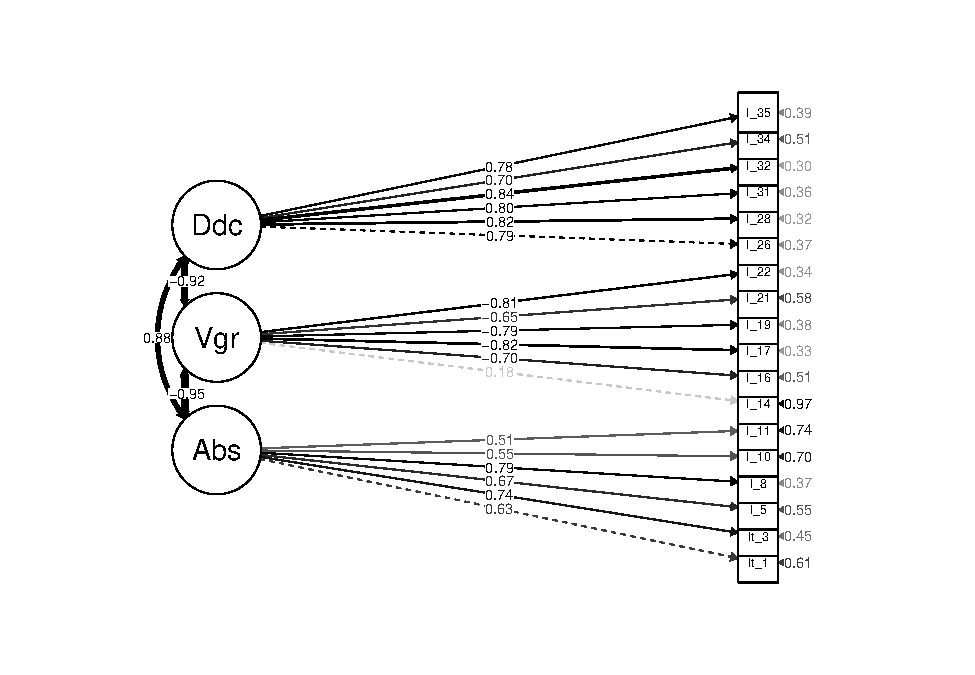
\includegraphics{EngagementPaper2_files/figure-latex/semplotsub-1.pdf}
\caption{\label{fig:semplotsub}Omnibus Confirmatory Factor Analysis substantive structure.}
\end{figure}

\begin{figure}
\centering
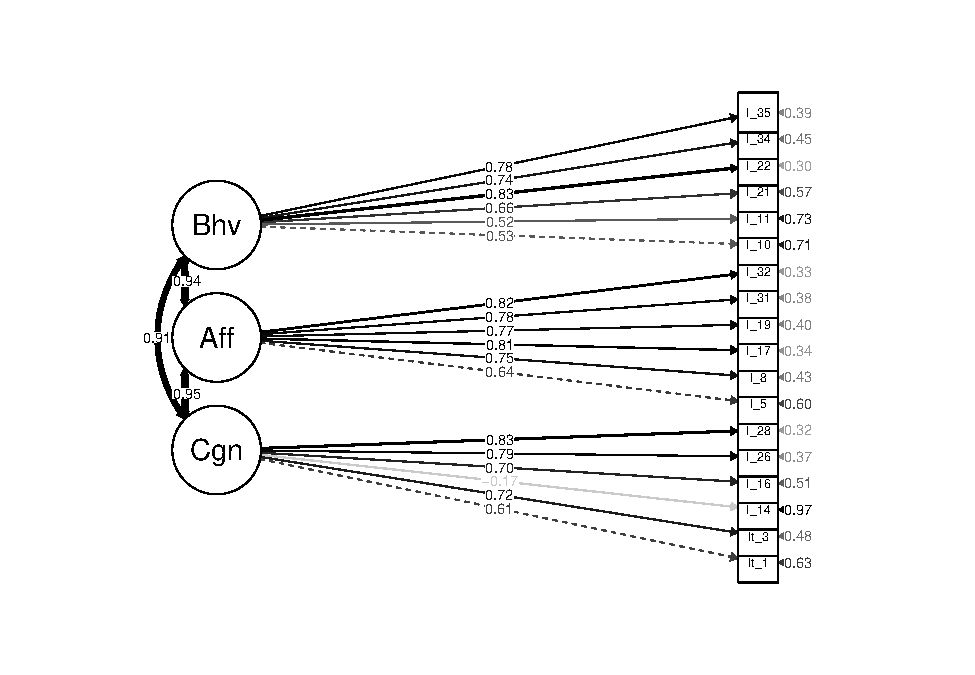
\includegraphics{EngagementPaper2_files/figure-latex/semplotatt-1.pdf}
\caption{\label{fig:semplotatt}Omnibus Confirmatory Factor Analysis attitudinal structure.}
\end{figure}

\begin{longtable}[]{@{}
  >{\raggedright\arraybackslash}p{(\columnwidth - 16\tabcolsep) * \real{0.0670}}
  >{\raggedright\arraybackslash}p{(\columnwidth - 16\tabcolsep) * \real{0.1453}}
  >{\raggedright\arraybackslash}p{(\columnwidth - 16\tabcolsep) * \real{0.1117}}
  >{\raggedright\arraybackslash}p{(\columnwidth - 16\tabcolsep) * \real{0.1229}}
  >{\raggedright\arraybackslash}p{(\columnwidth - 16\tabcolsep) * \real{0.1117}}
  >{\raggedright\arraybackslash}p{(\columnwidth - 16\tabcolsep) * \real{0.1117}}
  >{\raggedright\arraybackslash}p{(\columnwidth - 16\tabcolsep) * \real{0.1061}}
  >{\raggedright\arraybackslash}p{(\columnwidth - 16\tabcolsep) * \real{0.1117}}
  >{\raggedright\arraybackslash}p{(\columnwidth - 16\tabcolsep) * \real{0.1117}}@{}}
\toprule\noalign{}
\begin{minipage}[b]{\linewidth}\raggedright
Condition
\end{minipage} & \begin{minipage}[b]{\linewidth}\raggedright
Model
\end{minipage} & \begin{minipage}[b]{\linewidth}\raggedright
\(\chi^2\)
\end{minipage} & \begin{minipage}[b]{\linewidth}\raggedright
\emph{df}
\end{minipage} & \begin{minipage}[b]{\linewidth}\raggedright
RMSEA
\end{minipage} & \begin{minipage}[b]{\linewidth}\raggedright
SRMR
\end{minipage} & \begin{minipage}[b]{\linewidth}\raggedright
CFI
\end{minipage} & \begin{minipage}[b]{\linewidth}\raggedright
TLI
\end{minipage} & \begin{minipage}[b]{\linewidth}\raggedright
AIC
\end{minipage} \\
\midrule\noalign{}
\endhead
\bottomrule\noalign{}
\endlastfoot
Condition 1 & 3-factor substantive & 300.86 & 132 & 0.14 & 1 & 0.68 & 0.63 & 3,282.88 \\
& 3-factor attitudinal & 290.33 & 132 & 0.14 & 1 & 0.70 & 0.65 & 3,272.35 \\
Condition 2 & 3-factor substantive & 310.01 & 132 & 0.15 & 1 & 0.71 & 0.66 & 3,257.45 \\
& 3-factor attitudinal & 322.52 & 132 & 0.15 & 1 & 0.69 & 0.64 & 3,269.96 \\
Condition 3 & 3-factor substantive & 252.07 & 132 & 0.12 & 1 & 0.78 & 0.74 & 3,510.32 \\
& 3-factor attitudinal & 275.74 & 132 & 0.13 & 1 & 0.73 & 0.69 & 3534 \\
Condition 4 & 3-factor substantive & 224.96 & 132 & 0.10 & 0.94 & 0.82 & 0.79 & 3,421.64 \\
& 3-factor attitudinal & 228.99 & 132 & 0.10 & 0.96 & 0.81 & 0.78 & 3,425.66 \\
Condition 5 & 3-factor substantive & 549.80 & 132 & 0.10 & 1 & 0.90 & 0.89 & 14,932.57 \\
& 3-factor attitudinal & 497.90 & 132 & 0.10 & 1 & 0.92 & 0.90 & 14,880.67 \\
Condition 6 & 3-factor substantive & 468.02 & 132 & 0.09 & 0.87 & 0.91 & 0.90 & 17,953.02 \\
& 3-factor attitudinal & 610.60 & 132 & 0.10 & 1 & 0.88 & 0.86 & 18,095.61 \\
Overall & 3-factor substantive & 930.38 & 132 & 0.08 & 0.76 & 0.92 & 0.90 & 46,884.02 \\
& 3-factor attitudinal & 1,042.75 & 132 & 0.09 & 0.99 & 0.91 & 0.89 & 46,996.40 \\
\end{longtable}

\begin{lltable}

\begin{TableNotes}[para]
\normalsize{\textit{Note.} * p < 0.05; ** p < 0.01; *** p < 0.001}
\end{TableNotes}

\begin{longtable}{llllllll}\noalign{\getlongtablewidth\global\LTcapwidth=\longtablewidth}
\caption{\label{tab:unnamed-chunk-1}Unit-weighted scale intercorrelations (all conditions).}\\
\toprule
 & \multicolumn{1}{c}{1} & \multicolumn{1}{c}{2} & \multicolumn{1}{c}{3} & \multicolumn{1}{c}{4} & \multicolumn{1}{c}{5} & \multicolumn{1}{c}{$M$} & \multicolumn{1}{c}{$SD$}\\
\midrule
\endfirsthead
\caption*{\normalfont{Table \ref{tab:unnamed-chunk-1} continued}}\\
\toprule
 & \multicolumn{1}{c}{1} & \multicolumn{1}{c}{2} & \multicolumn{1}{c}{3} & \multicolumn{1}{c}{4} & \multicolumn{1}{c}{5} & \multicolumn{1}{c}{$M$} & \multicolumn{1}{c}{$SD$}\\
\midrule
\endhead
1. Absorption & - &  &  &  &  & 4.00 & 1.02\\
2. Vigor & .76*** & - &  &  &  & 4.22 & 0.85\\
3. Dedication & .76*** & .79*** & - &  &  & 4.41 & 1.12\\
4. Affect & .81*** & .83*** & .85*** & - &  & 4.08 & 0.90\\
5. Cognition & .87*** & .85*** & .89*** & .79*** & - & 4.16 & 1.12\\
6. Behavior & .84*** & .85*** & .84*** & .73*** & .81*** & 4.39 & 0.96\\
\bottomrule
\addlinespace
\insertTableNotes
\end{longtable}

\end{lltable}

\begin{quote}
Note. Also look at scale intercorrelations when the shared items have been removed (for example, items that define both dedication and cognition when looking at the correlation between dedication and cognition) - 12/2/21
\end{quote}

\hypertarget{condition-effects}{%
\subsubsection{Condition effects}\label{condition-effects}}

The order of item presentation was: 1) random within substantive dimension, 2) random within attitudinal dimension, 3) parcels of substantive within attitudinal (36-item attitudinal context), 4) parcels of attitudinal within substantive (36-item substantive context), 5) parcels of substantive within attitudinal (20-item attitudinal context), and 6) parcels of attitudinal within substantive (20-item substantive context). For example, in condition 1, the first items presented were all associated with one attitudinal dimension (for example, ``Affect''). Once the Affect item list was fully exhausted, the respondent was then administered the full set of Behavioral items, and once these were completed the respondent was then administered the Cognitive item set\footnote{Across conditions, the order of presentation of item ``blocks'' was also randomized. For example, not all respondents in Condition 1 was administered the Affect item block first - roughly 1/3 was presented the Behavioral block first and roughly 1/3 was presented the Cognitive block first.}. We view these orderings as cues regarding factor structure, and anticipated empirical factor structures to reflect these cues. The effects did emerge, but were quite moderate (for example, \(\Delta{\chi^2_{Cond1}}\) = 9.55, \(\Delta{AIC_{Cond1}}\) = 10.53). Given the variety of item orderings administered, this should be considered somewhat comforting regarding the effect of contextual embeddedness within multidimensional inventories. To further explore degree of similarity, we applied explicit tests of measurement invariance.

\hypertarget{measurement-invariance}{%
\paragraph{Measurement invariance}\label{measurement-invariance}}

Because our six conditions were obtained across two different sampling procedures, we apply our analyses of measurement invariance twice - first investigating the four conditions administered within our initial snowball sampling and then secondly also extending to the follow-up Qualtrics panel respondents.

We looked at structural invariance as well as latent means (Meredith, 1993; Steinmetz, Schmidt, Tina-Booh, Wieczorek, \& Schwartz, 2009).

\begin{table}[tbp]

\begin{center}
\begin{threeparttable}

\caption{\label{tab:measinv.pilot.att}Measurement invariance summary statistics (attitudinal structure).}

\begin{tabular}{lllllllll}
\toprule
 & \multicolumn{1}{c}{Df} & \multicolumn{1}{c}{AIC} & \multicolumn{1}{c}{BIC} & \multicolumn{1}{c}{Chisq} & \multicolumn{1}{c}{Chisq diff} & \multicolumn{1}{c}{RMSEA} & \multicolumn{1}{c}{Df diff} & \multicolumn{1}{c}{Pr(>Chisq)}\\
\midrule
configural.a & 528 & 13,645.98 & 14,453.38 & 1,117.59 & NA & NA & NA & NA\\
weak.a & 573 & 13,614.45 & 14,262.50 & 1,176.06 & 58.48 & 0.07 & 45 & 0.09\\
strong.a & 618 & 13,569.48 & 14,058.18 & 1,221.09 & 45.03 & 0.00 & 45 & 0.47\\
strict.a & 672 & 13,538.35 & 13,835.82 & 1,297.96 & 76.87 & 0.08 & 54 & 0.02\\
\bottomrule
\addlinespace
\end{tabular}

\begin{tablenotes}[para]
\normalsize{\textit{Note.} * p < 0.05; ** p < 0.01; *** p < 0.001}
\end{tablenotes}

\end{threeparttable}
\end{center}

\end{table}

\begin{table}[tbp]

\begin{center}
\begin{threeparttable}

\caption{\label{tab:measinv.pilot.sub}Measurement invariance summary statistics (substantive structure).}

\begin{tabular}{lllllllll}
\toprule
 & \multicolumn{1}{c}{Df} & \multicolumn{1}{c}{AIC} & \multicolumn{1}{c}{BIC} & \multicolumn{1}{c}{Chisq} & \multicolumn{1}{c}{Chisq diff} & \multicolumn{1}{c}{RMSEA} & \multicolumn{1}{c}{Df diff} & \multicolumn{1}{c}{Pr(>Chisq)}\\
\midrule
configural.s & 528 & 13,616.29 & 14,423.69 & 1,087.90 & NA & NA & NA & NA\\
weak.s & 573 & 13,588.39 & 14,236.44 & 1,150.00 & 62.10 & 0.08 & 45 & 0.05\\
strong.s & 618 & 13,546.51 & 14,035.20 & 1,198.12 & 48.12 & 0.03 & 45 & 0.35\\
strict.s & 672 & 13,521.28 & 13,818.74 & 1,280.89 & 82.77 & 0.09 & 54 & 0.01\\
\bottomrule
\addlinespace
\end{tabular}

\begin{tablenotes}[para]
\normalsize{\textit{Note.} * p < 0.05; ** p < 0.01; *** p < 0.001}
\end{tablenotes}

\end{threeparttable}
\end{center}

\end{table}

\begin{table}[tbp]

\begin{center}
\begin{threeparttable}

\caption{\label{tab:measinv.siop2.att}Measurement invariance summary statistics (attitudinal structure [6 conditions]).}

\begin{tabular}{lllllllll}
\toprule
 & \multicolumn{1}{c}{Df} & \multicolumn{1}{c}{AIC} & \multicolumn{1}{c}{BIC} & \multicolumn{1}{c}{Chisq} & \multicolumn{1}{c}{Chisq diff} & \multicolumn{1}{c}{RMSEA} & \multicolumn{1}{c}{Df diff} & \multicolumn{1}{c}{Pr(>Chisq)}\\
\midrule
configural.a2 & 792 & 46,694.26 & 48,335.92 & 2,226.09 & NA & NA & NA & NA\\
weak.a2 & 867 & 46,713.85 & 47,995.49 & 2,395.68 & 169.59 & 0.09 & 75 & 0.00\\
strong.a2 & 942 & 46,905.27 & 47,826.90 & 2,737.10 & 341.42 & 0.15 & 75 & 0.00\\
strict.a2 & 1032 & 46,946.38 & 47,436.00 & 2,958.21 & 221.11 & 0.10 & 90 & 0.00\\
\bottomrule
\addlinespace
\end{tabular}

\begin{tablenotes}[para]
\normalsize{\textit{Note.} * p < 0.05; ** p < 0.01; *** p < 0.001}
\end{tablenotes}

\end{threeparttable}
\end{center}

\end{table}

\hypertarget{discussion}{%
\section{Discussion}\label{discussion}}

Our contributions:

\begin{enumerate}
\def\labelenumi{\arabic{enumi}.}
\tightlist
\item
  Methodological
\end{enumerate}

\begin{itemize}
\tightlist
\item
  Intentional bi-factor structure
\end{itemize}

\begin{enumerate}
\def\labelenumi{\arabic{enumi}.}
\setcounter{enumi}{1}
\tightlist
\item
  Practical
\end{enumerate}

\begin{itemize}
\tightlist
\item
  A new public domain measure of engagement
\item
  Scalable to two aggregations (research {[}DAC{]} and actionable {[}ABC{]})
\end{itemize}

\begin{enumerate}
\def\labelenumi{\arabic{enumi}.}
\setcounter{enumi}{2}
\tightlist
\item
  Theoretical
\end{enumerate}

\begin{itemize}
\tightlist
\item
  Possibly help explain some of the high inter-scale correlations reported with other measures
\end{itemize}

The item cues did provide slight response cues (attending to individual model fit indices), however, the effect was quite small. Measurement invariance is plausible within our initial four administration conditions, although it is not attained across all six conditions. This is possibly attributable to differences in sampled population (in addition to the possibility that this difference is attributable to item orderings).

Our primary aspiration for developing this measure was that it would be a public domain instrument that would draw equal appeal from both practitioners and academics. These preliminary investigations suggest that it is scaleable to two aggregations which we have been referring to as: 1) research (DAC), and 2) actionable (ABC). Our (as-of-yet untested) assumption is that practitioners may be more interested in feedback regarding how their employees \emph{think}, \emph{feel}, and \emph{behave} with regard to engagement. Academics, on the other hand, may be more interested in possible differentiation between levels of dedication, absorption, and vigor. Having one assessment that may aggregate to either framework not only addresses the demand of constituent users, but it also facilitates aggregation across samplings for broader purposes such as norms development, validation, and metaanalysis.

The convergent indices provide preliminary evidence that the three engagement measures are measuring similar but not redundant content. The criterion-related indices suggest that the focal variable may have superior prediction, although more validation needs to occur, both with turnover intentions as well as actual turnover behavior. The disciminant validity indices did exhibit magnitudes slightly higher than anticipated, however, upon close inspection, the largest coefficients (\emph{r}'s of .15 and .17) emerged across the focal ``behavior'' and ``dedication'' scales. In retrospect, our sample respondents who engaged in more engagement behavior and exhibited higher levels of dedication could very well be expected to also extend those proclivities beyond work - perhaps including household and pet-care activities.

Although not explored here, there is also further predictive power potentially located within our intentionally complex instrument. It is possible that combined scale focus (for example, ``Cognitively Dedicated'' - shared items across the cognitive and dedication scales) exhibits even more predictive power for targeted outcomes of interest. Future investigations may wish to additionally probe for associations at this ``cell'' level.

\begin{tabular}{l|r|l|l|l}
\hline
name\_of\_sheet & num & oldest\_response & latest\_response & Sample\\
\hline
qualtrics\_pilot\_data.csv & 330 & 2020-11-15 09:43:31 & 2021-03-19 10:04:29 & Snowball sample from first go round using 2020 Eagle I.O cohort\\
\hline
Engagement+(Attitudinal)\_October+12,+2021\_08.02.csv & 341 & 2021-10-08 17:03:31 & 2021-10-12 07:40:25 & Samples comes from Renata's survey using 5 short measures of work engagement as well as free-time activities (spending time either with pets or game-playing). Ordering our measure using the attitudinal construct\\
\hline
Engagement+(Substantive)\_October+12,+2021\_08.01.csv & 402 & 2021-10-08 16:55:26 & 2021-10-11 17:10:21 & Samples comes from Renata's survey using 5 short measures of work engagement as well as free-time activities (spending time either with pets or game-playing). Ordering our measure using the substantive construct\\
\hline
inital\_data\_screen.csv & 281 & 2021-10-07 08:55:30 & 2021-10-07 15:40:41 & Sample comes from proflic data it is the inital sample. Everyone finish the survey in this sample.\\
\hline
inprogress.csv & 503 & 2021-10-07 08:46:48 & 2021-10-08 09:37:32 & Sample comes from proflic data it is the in progress sample. People did not finish the survey in this sample.\\
\hline
Engagement(post-Qualtrics)April1920221118.csv & 232 & 2021-10-27 10:27:49 & 2022-03-20 11:43:29 & Sample qualtrics after we remove 16 items. We also have the convergent and discriminant scaler on this survey\\
\hline
\end{tabular}

\newpage

\hypertarget{references}{%
\section{References}\label{references}}

\begingroup
\setlength{\parindent}{-0.5in}
\setlength{\leftskip}{0.5in}

\hypertarget{refs}{}
\begin{CSLReferences}{1}{0}
\leavevmode\vadjust pre{\hypertarget{ref-R-papaja}{}}%
Aust, F., \& Barth, M. (2020). \emph{{papaja}: {Create} {APA} manuscripts with {R Markdown}}. Retrieved from \url{https://github.com/crsh/papaja}

\leavevmode\vadjust pre{\hypertarget{ref-R-magrittr}{}}%
Bache, S. M., \& Wickham, H. (2020). \emph{Magrittr: A forward-pipe operator for r}. Retrieved from \url{https://CRAN.R-project.org/package=magrittr}

\leavevmode\vadjust pre{\hypertarget{ref-towersperrin2009}{}}%
Ballendowitsch, J., \& Perrin-ISR, T. (2009). Employee engagement--a way forward to productivity. \emph{Towers Perrin-ISR Case Study, Towers Perrin-ISR}, \emph{14}.

\leavevmode\vadjust pre{\hypertarget{ref-R-tinylabels}{}}%
Barth, M. (2022). \emph{{tinylabels}: Lightweight variable labels}. Retrieved from \url{https://cran.r-project.org/package=tinylabels}

\leavevmode\vadjust pre{\hypertarget{ref-baumruk2004missing}{}}%
Baumruk, R. (2004). \emph{The missing link: The role of employee engagement in business success}. \emph{47}, 48--52.

\leavevmode\vadjust pre{\hypertarget{ref-biderman2011ubiquity}{}}%
Biderman, M. D., Nguyen, N. T., Cunningham, C. J., \& Ghorbani, N. (2011). The ubiquity of common method variance: The case of the big five. \emph{Journal of Research in Personality}, \emph{45}(5), 417--429.

\leavevmode\vadjust pre{\hypertarget{ref-blessingwhite2018}{}}%
BlessingWhite. (2018). \emph{Employee engagement survey}. Available at \url{https://blessingwhite.com/wp-content/uploads/2019/11/Employee_Engagement_Survey_Fact_Sheet.pdf}.

\leavevmode\vadjust pre{\hypertarget{ref-coffman_hard_1999}{}}%
Coffman, C., \& Harter, J. (1999). A hard look at soft numbers. \emph{Position Paper, Gallup Organization}.

\leavevmode\vadjust pre{\hypertarget{ref-cole2012job}{}}%
Cole, M. S., Walter, F., Bedeian, A. G., \& O'Boyle, E. H. (2012). Job burnout and employee engagement: A meta-analytic examination of construct proliferation. \emph{Journal of Management}, \emph{38}(5), 1550--1581.

\leavevmode\vadjust pre{\hypertarget{ref-csikszentmihalyi1990flow}{}}%
Csikszentmihalyi, M. (1990). \emph{Flow: The psychology of optimal experience} (Vol. 1990). Harper \& Row New York.

\leavevmode\vadjust pre{\hypertarget{ref-elloy_examination_1991}{}}%
Elloy, D. F., Everett, J. E., \& Flynn, W. R. (1991). An examination of the correlates of job involvement. \emph{Group \& Organization Studies}, \emph{16}(2), 160--177. \url{https://doi.org/10.1177/105960119101600204}

\leavevmode\vadjust pre{\hypertarget{ref-R-semPlot}{}}%
Epskamp, S. (2019). \emph{semPlot: Path diagrams and visual analysis of various SEM packages' output}. Retrieved from \url{https://CRAN.R-project.org/package=semPlot}

\leavevmode\vadjust pre{\hypertarget{ref-ferris_added_1984}{}}%
Ferris, R., \& Hellier, P. (1984). Added value productivity schemes and employee participation. \emph{Asia Pacific Journal of Human Resources}, \emph{22}(4), 35--44. \url{https://doi.org/10.1177/103841118402200406}

\leavevmode\vadjust pre{\hypertarget{ref-R-sem}{}}%
Fox, J., Nie, Z., \& Byrnes, J. (2020). \emph{Sem: Structural equation models}. Retrieved from \url{https://CRAN.R-project.org/package=sem}

\leavevmode\vadjust pre{\hypertarget{ref-gade2017disentangling}{}}%
Gäde, J. C., Schermelleh-Engel, K., \& Klein, A. G. (2017). Disentangling the common variance of perfectionistic strivings and perfectionistic concerns: A bifactor model of perfectionism. \emph{Frontiers in Psychology}, \emph{8}, 160.

\leavevmode\vadjust pre{\hypertarget{ref-goering2017not}{}}%
Goering, D. D., Shimazu, A., Zhou, F., Wada, T., \& Sakai, R. (2017). Not if, but how they differ: A meta-analytic test of the nomological networks of burnout and engagement. \emph{Burnout Research}, \emph{5}, 21--34.

\leavevmode\vadjust pre{\hypertarget{ref-goldberg2010personality}{}}%
Goldberg, L. R. (2010). \emph{Then a miracle occurs: Focusing on behavior in social psychological theory and research} (C. R. Agnew, D. E. Carlston, W. G. Graziano, \& J. R. Kelly, Eds.). New York: Oxford University Press.

\leavevmode\vadjust pre{\hypertarget{ref-R-lubridate}{}}%
Grolemund, G., \& Wickham, H. (2011). Dates and times made easy with {lubridate}. \emph{Journal of Statistical Software}, \emph{40}(3), 1--25. Retrieved from \url{https://www.jstatsoft.org/v40/i03/}

\leavevmode\vadjust pre{\hypertarget{ref-harter_relationship_2013}{}}%
Harter, J. K., Schmidt, F. L., Agrawal, S., \& Plowman, S. K. (2013). The relationship between engagement at work and organizational outcomes 2012 Q12 meta-analysis lincoln. \emph{{NE}: The Gallup Organization}.

\leavevmode\vadjust pre{\hypertarget{ref-harter_business-unit-level_2002}{}}%
Harter, James K., Schmidt, F. L., \& Hayes, T. L. (2002). Business-unit-level relationship between employee satisfaction, employee engagement, and business outcomes: A meta-analysis. \emph{Journal of Applied Psychology}, \emph{87}(2), 268.

\leavevmode\vadjust pre{\hypertarget{ref-R-purrr}{}}%
Henry, L., \& Wickham, H. (2020). \emph{Purrr: Functional programming tools}. Retrieved from \url{https://CRAN.R-project.org/package=purrr}

\leavevmode\vadjust pre{\hypertarget{ref-hewitt2017}{}}%
Hewitt, A. (2017). \emph{2017 trends in global employee engagement}. Available at \url{https://content.lesaffaires.com/LAF/lacom/Aon_2017_Employee-Engagement.pdf}.

\leavevmode\vadjust pre{\hypertarget{ref-kahn1990psychological}{}}%
Kahn, William A. (1990b). Psychological conditions of personal engagement and disengagement at work. \emph{Academy of Management Journal}, \emph{33}(4), 692--724.

\leavevmode\vadjust pre{\hypertarget{ref-kahn_psychological_1990}{}}%
Kahn, William A. (1990a). Psychological conditions of personal engagement and disengagement at work. \emph{Academy of Management Journal}, \emph{33}(4), 692--724.

\leavevmode\vadjust pre{\hypertarget{ref-kaiser_campbell_2019}{}}%
Kaiser, F. G., \& Wilson, M. (2019). The {Campbell} {Paradigm} as a {Behavior}-{Predictive} {Reinterpretation} of the {Classical} {Tripartite} {Model} of {Attitudes}. \emph{European Psychologist}, \emph{24}(4), 359--374. \url{https://doi.org/10.1027/1016-9040/a000364}

\leavevmode\vadjust pre{\hypertarget{ref-kelloway1999source}{}}%
Kelloway, E. K., Gottlieb, B. H., \& Barham, L. (1999). The source, nature, and direction of work and family conflict: A longitudinal investigation. \emph{Journal of Occupational Health Psychology}, \emph{4}(4), 337--346.

\leavevmode\vadjust pre{\hypertarget{ref-kim_burnout_2009}{}}%
Kim, H. J., Shin, K. H., \& Swanger, N. (2009). Burnout and engagement: {A} comparative analysis using the {Big} {Five} personality dimensions. \emph{International Journal of Hospitality Management}, \emph{28}(1), 96--104. \url{https://doi.org/10.1016/j.ijhm.2008.06.001}

\leavevmode\vadjust pre{\hypertarget{ref-R-labourR}{}}%
Kouretsis, A., Bampouris, A., Morfiris, P., \& Papageorgiou, K. (2020). \emph{labourR: Classify multilingual labour market free-text to standardized hierarchical occupations}. Retrieved from \url{https://CRAN.R-project.org/package=labourR}

\leavevmode\vadjust pre{\hypertarget{ref-kulikowski2017we}{}}%
Kulikowski, K. (2017). Do we all agree on how to measure work engagement? Factorial validity of utrecht work engagement scale as a standard measurement tool--a literature review. \emph{International Journal of Occupational Medicine and Environmental Health}, \emph{30}(2), 161--175.

\leavevmode\vadjust pre{\hypertarget{ref-leiter_areas_2004}{}}%
Leiter, M., \& Maslach, C. (2004). Areas of worklife: A structured approach to organizational predictors of job burnout. In \emph{Research in occupational stress and well-being} (Vol. 3, pp. 91--134). \url{https://doi.org/10.1016/S1479-3555(03)03003-8}

\leavevmode\vadjust pre{\hypertarget{ref-leone_relation_1995}{}}%
Leone, D. R. (1995). \emph{The relation of work climate, higher order need satisfaction, need salience, and causality orientations to work engagement, psychological adjustment, and job satisfaction} (PhD thesis). ProQuest Information \& Learning.

\leavevmode\vadjust pre{\hypertarget{ref-maslach1997causes}{}}%
Maslach, C., \& Leiter, M. (1997). What causes burnout. \emph{Maslach C, Leiter MP. The Truth About Burnout: How Organizations Cause Personal Stress and What to Do about It. San Francisco, CA: Josey-Bass Publishers}, 38--60.

\leavevmode\vadjust pre{\hypertarget{ref-maslach_early_2008}{}}%
Maslach, Christina, \& Leiter, M. P. (2008). Early predictors of job burnout and engagement. \emph{Journal of Applied Psychology}, \emph{93}(3), 498--512.

\leavevmode\vadjust pre{\hypertarget{ref-meredith1993measurement}{}}%
Meredith, W. (1993). Measurement invariance, factor analysis and factorial invariance. \emph{Psychometrika}, \emph{58}(4), 525--543.

\leavevmode\vadjust pre{\hypertarget{ref-meyer_three-component_1991}{}}%
Meyer, J. P., \& Allen, N. J. (1991). A three-component conceptualization of organizational commitment. \emph{Human Resource Management Review}, \emph{1}(1), 61--89.

\leavevmode\vadjust pre{\hypertarget{ref-R-tibble}{}}%
Müller, K., \& Wickham, H. (2021). \emph{Tibble: Simple data frames}. Retrieved from \url{https://CRAN.R-project.org/package=tibble}

\leavevmode\vadjust pre{\hypertarget{ref-R-strex}{}}%
Nolan, R. (2023). \emph{Strex: Extra string manipulation functions}. Retrieved from \url{https://CRAN.R-project.org/package=strex}

\leavevmode\vadjust pre{\hypertarget{ref-R-base}{}}%
R Core Team. (2021). \emph{R: A language and environment for statistical computing}. Vienna, Austria: R Foundation for Statistical Computing. Retrieved from \url{https://www.R-project.org/}

\leavevmode\vadjust pre{\hypertarget{ref-reise_rediscovery_2012}{}}%
Reise, S. P. (2012). The rediscovery of bifactor measurement models. \emph{Multivariate Behavioral Research}, \emph{47}(5), 667--696. \url{https://doi.org/10.1080/00273171.2012.715555}

\leavevmode\vadjust pre{\hypertarget{ref-rosenberg_cognitive_1960}{}}%
Rosenberg, M. J. (1960). Cognitive, affective, and behavioral components of attitudes. In \emph{Attitude organization and change}.

\leavevmode\vadjust pre{\hypertarget{ref-R-lavaan}{}}%
Rosseel, Y. (2012). {lavaan}: An {R} package for structural equation modeling. \emph{Journal of Statistical Software}, \emph{48}(2), 1--36. Retrieved from \url{https://www.jstatsoft.org/v48/i02/}

\leavevmode\vadjust pre{\hypertarget{ref-engage_2022}{}}%
Russell, M., Ossorio Duffoo, C., Garcia Prieto Palacios Roji, R., \& Kulas, J. (2022). Development of an intentional bifactor measure of engagement. \emph{The Seattle Edition of SIOP}, 1--14. SIOP.

\leavevmode\vadjust pre{\hypertarget{ref-saks2006antecedents}{}}%
Saks, A. M. (2006). Antecedents and consequences of employee engagement. \emph{Journal of Managerial Psychology}, \emph{21}(7), 600--619.

\leavevmode\vadjust pre{\hypertarget{ref-saks2019antecedents}{}}%
Saks, A. M. (2019). Antecedents and consequences of employee engagement revisited. \emph{Journal of Organizational Effectiveness: People and Performance}, \emph{6}(1), 19--38.

\leavevmode\vadjust pre{\hypertarget{ref-schaufeli2013engagement}{}}%
Schaufeli, Wilmar B. (2013). What is engagement? In \emph{Employee engagement in theory and practice} (pp. 29--49). Routledge.

\leavevmode\vadjust pre{\hypertarget{ref-schaufeli_conceptualization_2010}{}}%
Schaufeli, Wilmar B., \& Bakker, A. (2010a). The conceptualization and measurement of work engagement. In Wilmar B. Schaufeli, A. Bakker, \& M. Leiter (Eds.), \emph{Work engagement: A handbook of essential theory and research} (pp. 10--24). New York: Psychology Press.

\leavevmode\vadjust pre{\hypertarget{ref-schaufeli_uwesutrecht_2003}{}}%
Schaufeli, W. B., \& Bakker, A. B. (2003). {UWES}--utrecht work engagement scale: Test manual. \emph{Unpublished Manuscript: Department of Psychology, Utrecht University}, \emph{8}.

\leavevmode\vadjust pre{\hypertarget{ref-schaufeli_defining_2010}{}}%
Schaufeli, Wilmar B., \& Bakker, A. B. (2010b). Defining and measuring work engagement: Bringing clarity to the concept. \emph{Work Engagement: A Handbook of Essential Theory and Research}, \emph{12}, 10--24.

\leavevmode\vadjust pre{\hypertarget{ref-schaufeli_measurement_2002}{}}%
Schaufeli, Wilmar B., Salanova, M., González-Romá, V., \& Bakker, A. B. (2002). The measurement of engagement and burnout: A two sample confirmatory factor analytic approach. \emph{Journal of Happiness Studies}, \emph{3}(1), 71--92.

\leavevmode\vadjust pre{\hypertarget{ref-schaufeli2008workaholism}{}}%
Schaufeli, Wilmar B., Taris, T. W., \& Van Rhenen, W. (2008). Workaholism, burnout, and work engagement: Three of a kind or three different kinds of employee well-being? \emph{Applied Psychology}, \emph{57}(2), 173--203.

\leavevmode\vadjust pre{\hypertarget{ref-shaw2005engagement}{}}%
Shaw, K. (2005). An engagement strategy process for communicators. \emph{Strategic Communication Management}, \emph{9}(3), 26.

\leavevmode\vadjust pre{\hypertarget{ref-sirota2013enthusiastic}{}}%
Sirota, D., \& Klein, D. (2013). \emph{The enthusiastic employee: How companies profit by giving workers what they want}. FT Press.

\leavevmode\vadjust pre{\hypertarget{ref-soane2012development}{}}%
Soane, E., Truss, C., Alfes, K., Shantz, A., Rees, C., \& Gatenby, M. (2012). Development and application of a new measure of employee engagement: The ISA engagement scale. \emph{Human Resource Development International}, \emph{15}(5), 529--547.

\leavevmode\vadjust pre{\hypertarget{ref-R-apaTables}{}}%
Stanley, D. (2021). \emph{apaTables: Create american psychological association (APA) style tables}. Retrieved from \url{https://CRAN.R-project.org/package=apaTables}

\leavevmode\vadjust pre{\hypertarget{ref-staw_employee_1994}{}}%
Staw, B. M., Sutton, R. I., \& Pelled, L. H. (1994). Employee positive emotion and favorable outcomes at the workplace. \emph{Organization Science}, \emph{5}(1), 51--71.

\leavevmode\vadjust pre{\hypertarget{ref-steinmetz2009testing}{}}%
Steinmetz, H., Schmidt, P., Tina-Booh, A., Wieczorek, S., \& Schwartz, S. H. (2009). Testing measurement invariance using multigroup CFA: Differences between educational groups in human values measurement. \emph{Quality \& Quantity}, \emph{43}(4), 599--616.

\leavevmode\vadjust pre{\hypertarget{ref-taris2017burnout}{}}%
Taris, T. W., Ybema, J. F., \& Beek, I. van. (2017). Burnout and engagement: Identical twins or just close relatives? \emph{Burnout Research}, \emph{5}, 3--11.

\leavevmode\vadjust pre{\hypertarget{ref-thackray_gallup_2005}{}}%
Thackray, J. (2005). \emph{The gallup Q12}. Gallup Management Journal.

\leavevmode\vadjust pre{\hypertarget{ref-timms2012burnt}{}}%
Timms, C., Brough, P., \& Graham, D. (2012). Burnt-out but engaged: The co-existence of psychological burnout and engagement. \emph{Journal of Educational Administration}, \emph{50}(3), 327--345.

\leavevmode\vadjust pre{\hypertarget{ref-R-ggplot2}{}}%
Wickham, H. (2016). \emph{ggplot2: Elegant graphics for data analysis}. Springer-Verlag New York. Retrieved from \url{https://ggplot2.tidyverse.org}

\leavevmode\vadjust pre{\hypertarget{ref-R-stringr}{}}%
Wickham, H. (2019). \emph{Stringr: Simple, consistent wrappers for common string operations}. Retrieved from \url{https://CRAN.R-project.org/package=stringr}

\leavevmode\vadjust pre{\hypertarget{ref-R-forcats}{}}%
Wickham, H. (2021a). \emph{Forcats: Tools for working with categorical variables (factors)}. Retrieved from \url{https://CRAN.R-project.org/package=forcats}

\leavevmode\vadjust pre{\hypertarget{ref-R-tidyr}{}}%
Wickham, H. (2021b). \emph{Tidyr: Tidy messy data}. Retrieved from \url{https://CRAN.R-project.org/package=tidyr}

\leavevmode\vadjust pre{\hypertarget{ref-R-tidyverse}{}}%
Wickham, H., Averick, M., Bryan, J., Chang, W., McGowan, L. D., François, R., \ldots{} Yutani, H. (2019). Welcome to the {tidyverse}. \emph{Journal of Open Source Software}, \emph{4}(43), 1686. \url{https://doi.org/10.21105/joss.01686}

\leavevmode\vadjust pre{\hypertarget{ref-R-dplyr}{}}%
Wickham, H., François, R., Henry, L., \& Müller, K. (2021). \emph{Dplyr: A grammar of data manipulation}. Retrieved from \url{https://CRAN.R-project.org/package=dplyr}

\leavevmode\vadjust pre{\hypertarget{ref-R-readr}{}}%
Wickham, H., \& Hester, J. (2020). \emph{Readr: Read rectangular text data}. Retrieved from \url{https://CRAN.R-project.org/package=readr}

\leavevmode\vadjust pre{\hypertarget{ref-R-knitr}{}}%
Xie, Y. (2015). \emph{Dynamic documents with {R} and knitr} (2nd ed.). Boca Raton, Florida: Chapman; Hall/CRC. Retrieved from \url{https://yihui.org/knitr/}

\leavevmode\vadjust pre{\hypertarget{ref-R-DT}{}}%
Xie, Y., Cheng, J., \& Tan, X. (2021). \emph{DT: A wrapper of the JavaScript library 'DataTables'}. Retrieved from \url{https://CRAN.R-project.org/package=DT}

\leavevmode\vadjust pre{\hypertarget{ref-R-kableExtra}{}}%
Zhu, H. (2021). \emph{kableExtra: Construct complex table with 'kable' and pipe syntax}. Retrieved from \url{https://CRAN.R-project.org/package=kableExtra}

\end{CSLReferences}

\endgroup


\end{document}
